% EN: \chapter{An Introduction to Inheritance and Polymorphism}
\Trans{\chapter{An Introduction to Inheritance and Polymorphism}}{\chapter{继承与多态简介}}

\textbf{C++} is, first and foremost, an object-oriented language, and objects are the fundamental building blocks of a C++ program. Class hierarchies are used to express relationships and interactions between different parts of a software system, define and implement interfaces between components, and organize data and code. While this isn't a book for teaching C++, the aim of this chapter is to give the reader enough knowledge about C++ language features as they relate to classes and inheritance, which will be used in later chapters. To that end, we won't attempt to completely describe the C++ tools for working with classes but introduce the concepts and language constructs that will be used throughout this book.

% EN: The following topics will be covered in this chapter:
\Trans{The following topics will be covered in this chapter:}{本章将讨论以下主题:}

\begin{itemize}
\item
% EN:   What are classes and what is their role in C++?
\Trans{What are classes and what is their role in C++?}{什么是类?它们在 C++ 中承担什么角色?}
\item
% EN:   What are class hierarchies and how does C++ use inheritance?
\Trans{What are class hierarchies and how does C++ use inheritance?}{什么是类层次结构?C++ 如何利用继承?}
\item
% EN:   What is runtime polymorphism and how is it used in C++?
\Trans{What is runtime polymorphism and how is it used in C++?}{什么是运行时多态?它在 C++ 中怎样被使用?}
\end{itemize}

\section{Classes and objects}

% EN: Object-oriented programming is a way to structure a program by combining the algorithms and the data that the algorithms operate on into single entities called \textbf{objects}. Most object-oriented languages, including C++, are class-based. A \textbf{class} is a definition of an object---it describes the algorithms and the data, its format, and its relations to other classes. An object is a concrete instantiation of a class, that is, a variable. An object has an address, which is a location in memory. A class is a user-defined type. In general, any number of objects can be instantiated from the definition provided by the class (some classes limit the number of objects that can be created, but this is an exception, not the norm).
\Trans{Object-oriented programming is a way to structure a program by combining the algorithms and the data that the algorithms operate on into single entities called \textbf{objects}. Most object-oriented languages, including C++, are class-based. A \textbf{class} is a definition of an object---it describes the algorithms and the data, its format, and its relations to other classes. An object is a concrete instantiation of a class, that is, a variable. An object has an address, which is a location in memory. A class is a user-defined type. In general, any number of objects can be instantiated from the definition provided by the class (some classes limit the number of objects that can be created, but this is an exception, not the norm).}{面向对象编程是一种组织程序的方式:将算法以及这些算法所操作的数据结合为单一实体,称为\textbf{对象}。多数面向对象语言(包括 C++)都是“以类为中心”的。\textbf{类} 是对象的定义——它描述算法与数据、它们的表达形式,以及与其他类的关系。对象是类的一个具体实例,也就是一个变量。对象在内存中有一个地址。类是用户自定义类型。通常情况下,可以根据类的定义实例化任意数量的对象(某些类会限制可创建对象的数量,但那只是特例而非常规)。}

% EN: In C++, the data contained in a class is organized as a collection of data members, or variables, of different types. The algorithms are implemented as functions---the methods of the class. While there's no language requirement that the data members of a class should be somehow relevant to the implementation of its methods, it's one of the signs of good design when the data is well encapsulated in the classes, and the methods have limited interaction with external data.
\Trans{In C++, the data contained in a class is organized as a collection of data members, or variables, of different types. The algorithms are implemented as functions---the methods of the class. While there's no language requirement that the data members of a class should be somehow relevant to the implementation of its methods, it's one of the signs of good design when the data is well encapsulated in the classes, and the methods have limited interaction with external data.}{}

% EN: This concept of \textbf{encapsulation} is central to the classes in C++---the language allows us to control which data members and methods are public---visible outside of the class, and which are internal---private to the class. A well-designed class has mostly, or only, private data members, and the only public methods are those needed to express the public interface of the class---in other words, what the class does. This public interface is like a contract---the class designer promises that this class provides certain features and operations. The private data and methods of the class are part of the implementation, and they can be changed as long as the public interface, the contract we've committed to, remains valid. For example, the following class represents a rational number and supports the increment operation, as exposed by its public interface:
\Trans{This concept of \textbf{encapsulation} is central to the classes in C++---the language allows us to control which data members and methods are public---visible outside of the class, and which are internal---private to the class. A well-designed class has mostly, or only, private data members, and the only public methods are those needed to express the public interface of the class---in other words, what the class does. This public interface is like a contract---the class designer promises that this class provides certain features and operations. The private data and methods of the class are part of the implementation, and they can be changed as long as the public interface, the contract we've committed to, remains valid. For example, the following class represents a rational number and supports the increment operation, as exposed by its public interface:}{}

\begin{code}
% EN: class Rational { public:
  Rational& operator+=(const Rational& rhs);
 };
\Trans{class Rational { public: Rational& operator+=(const Rational& rhs); };}{}

\end{code}

% EN: A well-designed class doesn't expose any more of the implementation details than it has to through its public interface. The implementation isn't part of the contract, although the documented interface may impose some restrictions on it. For example, if we promise that all rational numbers don't contain any common multipliers in the numerator and denomination, the addition should include the step of canceling them. That would be a good use of a private member function---the implementation of several other operations will need to call it, but the client of the class never needs to call it because every rational number is already reduced to its lowest terms before it's exposed to the callers:
\Trans{A well-designed class doesn't expose any more of the implementation details than it has to through its public interface. The implementation isn't part of the contract, although the documented interface may impose some restrictions on it. For example, if we promise that all rational numbers don't contain any common multipliers in the numerator and denomination, the addition should include the step of canceling them. That would be a good use of a private member function---the implementation of several other operations will need to call it, but the client of the class never needs to call it because every rational number is already reduced to its lowest terms before it's exposed to the callers:}{}

\begin{code}
% EN: class Rational {
  public:
  Rational& operator+=(const Rational& rhs); private:
  long n_; // numerator
  long d_; // denominator
  void  reduce();
 };
Rational& Rational::operator+=(const Rational& rhs) {
  n_ = n_*rhs.d_ + rhs.n_*d_;
  d_ = d_*rhs.d_; reduce();
  return *this;
\Trans{class Rational { public: Rational& operator+=(const Rational& rhs); private: long n_; // numerator long d_; // denominator void reduce(); }; Rational& Rational::operator+=(const Rational& rhs) { n_ = n_*rhs.d_ + rhs.n_*d_; d_ = d_*rhs.d_; reduce(); return *this;}{}

}
% EN: Rational a, b; a += b;
\Trans{Rational a, b; a += b;}{}
\end{code}

% EN: The class methods have special access to the data members---they can access the private data of the class. Note the distinction between the class and the object here---\texttt{operator+=()} is a method of the \texttt{Rational} class and is invoked on the object, \texttt{a}. However, it has access to the private data of the \texttt{b} object as well, because \texttt{a} and \texttt{b} are objects of the same class. If a member function references a class member by name without any additional qualifiers, then it's accessing a member of the same class it's invoked on (we can make it explicit by writing \texttt{this-\textgreater{}n\_} and \texttt{this-\textgreater{}d\_}). Accessing members of another object of the same class requires a pointer or a reference to that object, but is otherwise not restricted, as would have been the case if we tried to access a private data member from a non-member function.
\Trans{The class methods have special access to the data members---they can access the private data of the class. Note the distinction between the class and the object here---\texttt{operator+=()} is a method of the \texttt{Rational} class and is invoked on the object, \texttt{a}. However, it has access to the private data of the \texttt{b} object as well, because \texttt{a} and \texttt{b} are objects of the same class. If a member function references a class member by name without any additional qualifiers, then it's accessing a member of the same class it's invoked on (we can make it explicit by writing \texttt{this-\textgreater{}n\_} and \texttt{this-\textgreater{}d\_}). Accessing members of another object of the same class requires a pointer or a reference to that object, but is otherwise not restricted, as would have been the case if we tried to access a private data member from a non-member function.}{}

% EN: By the way, C++ also supports C-style structs. But in C++, a struct isn't limited to just an aggregate of data members---it can have methods, public and private access modifiers, and anything else classes have. From a language point of view, the only difference between a class and a struct is the default access---in a class, all members and methods are private by default, while in a struct they're public. Beyond that, the use of structs instead of classes is a matter of convention---traditionally, structs are used for C-style structs (structs that would be legal in C) as well as \emph{almost} C-style structs, for example, a struct with only a constructor added. Of course, this boundary isn't precise and is a matter of coding styles and practices in each project or team.
\Trans{By the way, C++ also supports C-style structs. But in C++, a struct isn't limited to just an aggregate of data members---it can have methods, public and private access modifiers, and anything else classes have. From a language point of view, the only difference between a class and a struct is the default access---in a class, all members and methods are private by default, while in a struct they're public. Beyond that, the use of structs instead of classes is a matter of convention---traditionally, structs are used for C-style structs (structs that would be legal in C) as well as \emph{almost} C-style structs, for example, a struct with only a constructor added. Of course, this boundary isn't precise and is a matter of coding styles and practices in each project or team.}{}

% EN: In addition to the methods and data members we've seen, C++ also supports static data and methods. A static method is very similar to a regular non-member function---it isn't invoked on any particular object, and the only way it can get access to an object of any type is through its arguments. However, unlike a non-member function, a static method retains its privileged access to the private data of the class.
\Trans{In addition to the methods and data members we've seen, C++ also supports static data and methods. A static method is very similar to a regular non-member function---it isn't invoked on any particular object, and the only way it can get access to an object of any type is through its arguments. However, unlike a non-member function, a static method retains its privileged access to the private data of the class.}{}

% EN: Classes by themselves are a useful way to group together (encapsulate) the algorithms and the data they operate on and to limit access to some data. However, the most powerful object-oriented features of C++ are inheritance and the resulting class hierarchies.
\Trans{Classes by themselves are a useful way to group together (encapsulate) the algorithms and the data they operate on and to limit access to some data. However, the most powerful object-oriented features of C++ are inheritance and the resulting class hierarchies.}{}

\section{Inheritance and class hierarchies}

% EN: Class hierarchies in C++ serve a dual purpose. On the one hand, they allow us to express relations between objects. On the other hand, they let us compose more complex types from simpler ones. Both uses are accomplished through inheritance.
\Trans{Class hierarchies in C++ serve a dual purpose. On the one hand, they allow us to express relations between objects. On the other hand, they let us compose more complex types from simpler ones. Both uses are accomplished through inheritance.}{}

% EN: The concept of inheritance is central to the C++ use of classes and objects. Inheritance allows us to define new classes as extensions of existing ones. When a derived class is inherited from the base class, it contains, in some form, all of the data and the algorithms that were in the base class, and it adds some of its own. In C++, it's important to distinguish between two primary types of inheritance---public and private.
\Trans{The concept of inheritance is central to the C++ use of classes and objects. Inheritance allows us to define new classes as extensions of existing ones. When a derived class is inherited from the base class, it contains, in some form, all of the data and the algorithms that were in the base class, and it adds some of its own. In C++, it's important to distinguish between two primary types of inheritance---public and private.}{}

% EN: Public inheritance inherits the public interface of the class. It also inherits the implementation---the data members of the base class are also a part of the derived class. But the inheritance of the interface is what distinguishes public inheritance---the derived class has, as a part of its public interface, the public member functions of the base class.
\Trans{Public inheritance inherits the public interface of the class. It also inherits the implementation---the data members of the base class are also a part of the derived class. But the inheritance of the interface is what distinguishes public inheritance---the derived class has, as a part of its public interface, the public member functions of the base class.}{}

% EN: Remember that the public interface is like a contract---we promise to the clients of the class that it supports certain operations, maintains some invariants, and obeys the specified restrictions. By publicly inheriting from the base class, we bind the derived class to the same contract (plus any extensions of the contract, should we decide to define additional public interfaces). Because the derived class also respects the interface contract of the base class, we could use a derived class in any place in the code where a base class is expected---we would not be able to use any of the extensions to the interface (the code expects the base class, we don't know about any extensions at that point), but the base class interface and its restrictions have to be valid.
\Trans{Remember that the public interface is like a contract---we promise to the clients of the class that it supports certain operations, maintains some invariants, and obeys the specified restrictions. By publicly inheriting from the base class, we bind the derived class to the same contract (plus any extensions of the contract, should we decide to define additional public interfaces). Because the derived class also respects the interface contract of the base class, we could use a derived class in any place in the code where a base class is expected---we would not be able to use any of the extensions to the interface (the code expects the base class, we don't know about any extensions at that point), but the base class interface and its restrictions have to be valid.}{}

% EN: This is often expressed as the \emph{is-a principle}---an instance of a derived class is also an instance of the base class. However, the way we interpret the \emph{is-a} relationship in C++ isn't exactly intuitive. For example, is a square a rectangle? If it is, then we can derive the \texttt{Square} class from the \texttt{Rectangle} class:
\Trans{This is often expressed as the \emph{is-a principle}---an instance of a derived class is also an instance of the base class. However, the way we interpret the \emph{is-a} relationship in C++ isn't exactly intuitive. For example, is a square a rectangle? If it is, then we can derive the \texttt{Square} class from the \texttt{Rectangle} class:}{}

\begin{code}
% EN: class Rectangle {
  public:
  double Length() const { return length_;  }
  double Width() const { return width_;  }
  ...
  private:
  double l_;
  double w_;
 };
class Square : public Rectangle {
  ...
 };
\Trans{class Rectangle { public: double Length() const { return length_; } double Width() const { return width_; } ... private: double l_; double w_; }; class Square : public Rectangle { ... };}{}

\end{code}

% EN: Right away, there's something that doesn't seem right---the derived class has two data members for dimensions, but it really needs only one. We would have to somehow enforce that they're always the same. This doesn't seem so bad---the \texttt{Rectangle} class has the interface that allows for any positive values of length and width, and the \texttt{Square} imposes additional restrictions. But it's worse than that---the \texttt{Rectangle} class has a contract that allows the user to make the dimensions different. This can be quite explicit:
\Trans{Right away, there's something that doesn't seem right---the derived class has two data members for dimensions, but it really needs only one. We would have to somehow enforce that they're always the same. This doesn't seem so bad---the \texttt{Rectangle} class has the interface that allows for any positive values of length and width, and the \texttt{Square} imposes additional restrictions. But it's worse than that---the \texttt{Rectangle} class has a contract that allows the user to make the dimensions different. This can be quite explicit:}{}

\begin{code}
% EN: class Rectangle {
  public:
  void Scale(double sl, double sw) {
     // Scale the dimensions
    length_ *= sl;
    width_ *= sw;
   }
  ...
 };
\Trans{class Rectangle { public: void Scale(double sl, double sw) { // Scale the dimensions length_ *= sl; width_ *= sw; } ... };}{}

\end{code}

% EN: Now, we have a public method that allows us to distort the rectangle, altering its aspect ratio. As with any other public method, it's inherited by the derived classes, so now the \texttt{Square} class has it too. In fact, by using public inheritance, we assert that a \texttt{Square} object can be used anywhere a \texttt{Rectangle} object is used, without even knowing that it's really a \texttt{Square}. Clearly, this is a promise we can't keep---when the client of our class hierarchy tries to change the aspect ratio of a square, we can't do it. We could ignore the call or report an error at runtime. Either way, we've violated the contract provided by the base class. There's only one solution---in C++, a square isn't a rectangle. Note that a rectangle is usually not a square, either---the contract provided by the \texttt{Square} interface could contain any number of guarantees that we can't maintain if we derive the \texttt{Rectangle} class from \texttt{Square}.
\Trans{Now, we have a public method that allows us to distort the rectangle, altering its aspect ratio. As with any other public method, it's inherited by the derived classes, so now the \texttt{Square} class has it too. In fact, by using public inheritance, we assert that a \texttt{Square} object can be used anywhere a \texttt{Rectangle} object is used, without even knowing that it's really a \texttt{Square}. Clearly, this is a promise we can't keep---when the client of our class hierarchy tries to change the aspect ratio of a square, we can't do it. We could ignore the call or report an error at runtime. Either way, we've violated the contract provided by the base class. There's only one solution---in C++, a square isn't a rectangle. Note that a rectangle is usually not a square, either---the contract provided by the \texttt{Square} interface could contain any number of guarantees that we can't maintain if we derive the \texttt{Rectangle} class from \texttt{Square}.}{}

% EN: Similarly, a penguin isn't a bird in C++ if the bird interface includes flying. The correct design for such cases usually includes a more abstract base class, \texttt{Bird}, that doesn't make any promises that at least one derived class can't keep (for example, a \texttt{Bird} object doesn't make a guarantee that it can fly). Then, we create intermediate-based classes, such as \texttt{FlyingBird} and \texttt{FlightlessBird}, that are derived from the common base class and serve as base classes for the more specific classes such as \texttt{Eagle} or \texttt{Penguin}. The important lesson here is that whether or not a penguin is a bird in C++ depends on how we define what a bird is, or, in C++ terms, what the public interface of the \texttt{Bird} class is.
\Trans{Similarly, a penguin isn't a bird in C++ if the bird interface includes flying. The correct design for such cases usually includes a more abstract base class, \texttt{Bird}, that doesn't make any promises that at least one derived class can't keep (for example, a \texttt{Bird} object doesn't make a guarantee that it can fly). Then, we create intermediate-based classes, such as \texttt{FlyingBird} and \texttt{FlightlessBird}, that are derived from the common base class and serve as base classes for the more specific classes such as \texttt{Eagle} or \texttt{Penguin}. The important lesson here is that whether or not a penguin is a bird in C++ depends on how we define what a bird is, or, in C++ terms, what the public interface of the \texttt{Bird} class is.}{}

% EN: Because the public inheritance implies the \emph{is-a} relationship, the language allows a wide range of conversions between references and pointers to different classes in the same hierarchy. First of all, a conversion from a pointer to a derived class into a pointer to the base class is implicit (this is the same for references):
\Trans{Because the public inheritance implies the \emph{is-a} relationship, the language allows a wide range of conversions between references and pointers to different classes in the same hierarchy. First of all, a conversion from a pointer to a derived class into a pointer to the base class is implicit (this is the same for references):}{}

\begin{code}
% EN: class Base { ...  };
class Derived : public Base { ...  };
Derived* d = new Derived;
Base* b = d;    // Implicit conversion
\Trans{class Base { ... }; class Derived : public Base { ... }; Derived* d = new Derived; Base* b = d; // Implicit conversion}{}

\end{code}

% EN: This conversion is always valid because an instance of the derived class is also an instance of the base class. The inverse conversion is possible but has to be made explicit:
\Trans{This conversion is always valid because an instance of the derived class is also an instance of the base class. The inverse conversion is possible but has to be made explicit:}{}

\begin{code}
% EN: Base* b = new Derived;     // *b is really Derived
Derived* d = b; // Does not compile, not implicit Derived*
Derived* d1 =
     static_cast<Derived*>(b);    // Explicit conversion
\Trans{Base* b = new Derived; // *b is really Derived Derived* d = b; // Does not compile, not implicit Derived* Derived* d1 = static_cast<Derived*>(b); // Explicit conversion}{}

\end{code}

% EN: The reason this conversion isn't implicit is that it's valid only if the base class pointer really points to a derived object (otherwise, the behavior is undefined). The programmer, therefore, must explicitly assert, using the static cast, that somehow, through the logic of the program or a prior test or by some other means, it's known that this conversion is valid. If you aren't sure that the conversion is valid, there's a safer way to try it without causing undefined behavior; we'll learn about this in the next section.
\Trans{The reason this conversion isn't implicit is that it's valid only if the base class pointer really points to a derived object (otherwise, the behavior is undefined). The programmer, therefore, must explicitly assert, using the static cast, that somehow, through the logic of the program or a prior test or by some other means, it's known that this conversion is valid. If you aren't sure that the conversion is valid, there's a safer way to try it without causing undefined behavior; we'll learn about this in the next section.}{}

% EN: Note that the static (or implicit) conversion between pointers to base and derived classes is not quite as straightforward as you might think. The first base of any object always has the same address as the derived object itself, but then it gets more complicated. There is generally no standard requirement on the memory layout of derived classes with multiple bases:
\Trans{Note that the static (or implicit) conversion between pointers to base and derived classes is not quite as straightforward as you might think. The first base of any object always has the same address as the derived object itself, but then it gets more complicated. There is generally no standard requirement on the memory layout of derived classes with multiple bases:}{}

\begin{code}
% EN: class Base1 { ...  };
class Base2 { ...  };
class Derived : public Base1, public Base2 { ...  };
\Trans{class Base1 { ... }; class Base2 { ... }; class Derived : public Base1, public Base2 { ... };}{}

\end{code}

% EN: Most compilers will lay out the base classes first, then the data members of the derived class:
\Trans{Most compilers will lay out the base classes first, then the data members of the derived class:}{}

\pandocbounded{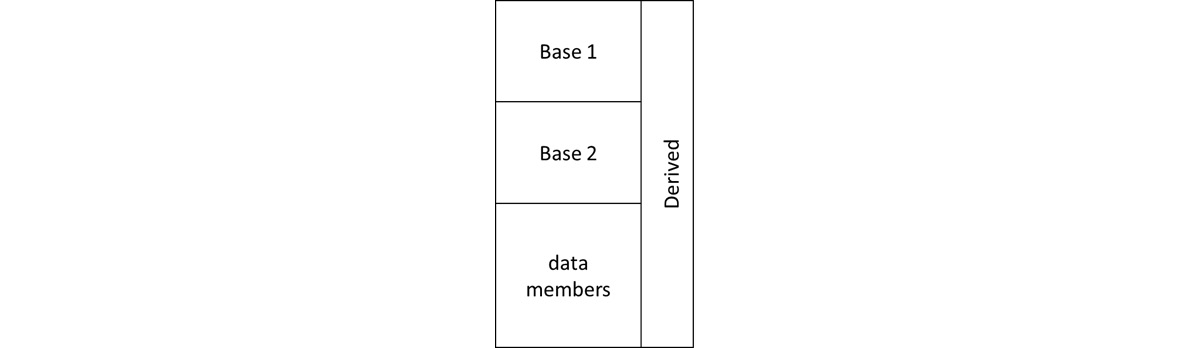
\includegraphics[keepaspectratio]{./image/Figure_1.1_B19262.jpg}}

% EN: Figure 1.1 -- Possible memory layout of a derived class
\Trans{Figure 1.1 -- Possible memory layout of a derived class}{}

% EN: From \emph{Figure 1.1}, it is evident that pointer conversion between the base and derived classes generally involves offset calculations. We can easily see this in an example:
\Trans{From \emph{Figure 1.1}, it is evident that pointer conversion between the base and derived classes generally involves offset calculations. We can easily see this in an example:}{}

\begin{code}
% EN: // Example 01_cast.C
Derived d;
Derived* p = &d;
std::cout << "Derived: " << (void*)(p) <<
  " Base1: " << (void*)(static_cast<Base1*>(p)) <<
  " Base2: " << (void*)(static_cast<Base2*>(p)) <<
  std::endl;
\Trans{// Example 01_cast.C Derived d; Derived* p = &d; std::cout << "Derived: " << (void*)(p) << " Base1: " << (void*)(static_cast<Base1*>(p)) << " Base2: " << (void*)(static_cast<Base2*>(p)) << std::endl;}{}

\end{code}

% EN: The program prints something like this:
\Trans{The program prints something like this:}{}

\begin{code}
% EN: Derived: 0x7f97e550 Base1: 0x7f97e550 Base2: 0x7f97e560
\Trans{Derived: 0x7f97e550 Base1: 0x7f97e550 Base2: 0x7f97e560}{}
\end{code}

% EN: You can see that the \texttt{Base1} object is located at the same address as the \texttt{Derived} object, and \texttt{Base2} starts with an offset (16 bytes, in our case). Seems like the cast is an easy calculation: If you have a pointer to \texttt{Derived} and you want to cast to \texttt{Base2}, add 16. The offsets between base classes are known at compile time, and the compiler knows the layout it is using. Pointer offset calculations are usually implemented in hardware (all modern CPUs support them and do not require a separate addition instruction). This doesn't sound so hard at all.
\Trans{You can see that the \texttt{Base1} object is located at the same address as the \texttt{Derived} object, and \texttt{Base2} starts with an offset (16 bytes, in our case). Seems like the cast is an easy calculation: If you have a pointer to \texttt{Derived} and you want to cast to \texttt{Base2}, add 16. The offsets between base classes are known at compile time, and the compiler knows the layout it is using. Pointer offset calculations are usually implemented in hardware (all modern CPUs support them and do not require a separate addition instruction). This doesn't sound so hard at all.}{}

% EN: Now, what do you do if the pointer is \texttt{null}? The pointer has a value of 0. If you apply the same \emph{conversion}, you get \texttt{16\ (0x10)}, and now your check for \texttt{null} fails:
\Trans{Now, what do you do if the pointer is \texttt{null}? The pointer has a value of 0. If you apply the same \emph{conversion}, you get \texttt{16\ (0x10)}, and now your check for \texttt{null} fails:}{}

\begin{code}
% EN: void f(Base2* p) {
  if (p != nullptr) do_work(*p);
\Trans{void f(Base2* p) { if (p != nullptr) do_work(*p);}{}

}
% EN: Derived* p = nullptr;
f(p); // Will it try to dereference 0x10?
\Trans{Derived* p = nullptr; f(p); // Will it try to dereference 0x10?}{}

\end{code}

% EN: Obviously, this would be very bad, so we can assume that \texttt{null} pointers remain so. Indeed, they do:
\Trans{Obviously, this would be very bad, so we can assume that \texttt{null} pointers remain so. Indeed, they do:}{}

\begin{code}
% EN: Derived* p = nullptr;
std::cout << "Derived: " << (void*)(p) <<
  " Base1: " << (void*)(static_cast<Base1*>(p)) <<
  " Base2: " << (void*)(static_cast<Base2*>(p)) <<
  std::endl;
\Trans{Derived* p = nullptr; std::cout << "Derived: " << (void*)(p) << " Base1: " << (void*)(static_cast<Base1*>(p)) << " Base2: " << (void*)(static_cast<Base2*>(p)) << std::endl;}{}

\end{code}

% EN: This prints the same values for all pointers:
\Trans{This prints the same values for all pointers:}{}

\begin{code}
% EN: Derived: 0x0 Base1: 0x0 Base2: 0x0
\Trans{Derived: 0x0 Base1: 0x0 Base2: 0x0}{}
\end{code}

% EN: This is the only way to do casts, but it implies that a simple implicit cast from \texttt{Derived*} to \texttt{Base*} hides inside a conditional computation with a \texttt{null} pointer check.
\Trans{This is the only way to do casts, but it implies that a simple implicit cast from \texttt{Derived*} to \texttt{Base*} hides inside a conditional computation with a \texttt{null} pointer check.}{}

% EN: The other kind of inheritance in C++ is \textbf{private inheritance}. When inheriting privately, the derived classes don't extend the public interface of the base class---all base class methods become private in the derived class. Any public interface has to be created by the derived class, starting from a clean slate. There's no assumption that an object of the derived class can be used in place of an object of the base class. What the derived class does get from the base class is the implementation details---both the methods and the data members can be used by the derived class to implement its own algorithms. It's said, therefore, that private inheritance implements a \emph{has-a} relationship---the derived object has an instance of the base class contained inside of it.
\Trans{The other kind of inheritance in C++ is \textbf{private inheritance}. When inheriting privately, the derived classes don't extend the public interface of the base class---all base class methods become private in the derived class. Any public interface has to be created by the derived class, starting from a clean slate. There's no assumption that an object of the derived class can be used in place of an object of the base class. What the derived class does get from the base class is the implementation details---both the methods and the data members can be used by the derived class to implement its own algorithms. It's said, therefore, that private inheritance implements a \emph{has-a} relationship---the derived object has an instance of the base class contained inside of it.}{}

% EN: The relation of the privately derived class to its base class is, therefore, similar to that of the relationship of a class to its data members. The latter implementation technique is known as \textbf{composition}---an object is composed of any number of other objects, which are all used as its data members. In the absence of any reason to do otherwise, the composition should be preferred to private inheritance. What, then, might be the reasons to use private inheritance? There are several possibilities. First of all, it's possible, within the derived class, to re-expose one of the public member functions of the base class with the help of a \texttt{using} declaration:
\Trans{The relation of the privately derived class to its base class is, therefore, similar to that of the relationship of a class to its data members. The latter implementation technique is known as \textbf{composition}---an object is composed of any number of other objects, which are all used as its data members. In the absence of any reason to do otherwise, the composition should be preferred to private inheritance. What, then, might be the reasons to use private inheritance? There are several possibilities. First of all, it's possible, within the derived class, to re-expose one of the public member functions of the base class with the help of a \texttt{using} declaration:}{}

\begin{code}
% EN: class Container : private std::vector<int> {
  public:
  using std::vector<int>::size;
  ...
 };
\Trans{class Container : private std::vector<int> { public: using std::vector<int>::size; ... };}{}

\end{code}

% EN: This can be useful in rare cases, but it's also equivalent to an inline forwarding function:
\Trans{This can be useful in rare cases, but it's also equivalent to an inline forwarding function:}{}

\begin{code}
% EN: class Container {
  private:
  std::vector<int> v_;
  public:
  size_t size() const { return v_.size();  }
  ...
 };
\Trans{class Container { private: std::vector<int> v_; public: size_t size() const { return v_.size(); } ... };}{}

\end{code}

% EN: Second, a pointer or reference to a derived object can be converted into a pointer or reference to the base object, but only inside a member function of the derived class. Again, the equivalent functionality for composition is provided by taking the address of a data member. So far, we haven't seen a good reason to use private inheritance, and indeed, the common advice is to prefer composition. But the next two reasons are more significant, and either one could be motivation enough to use private inheritance.
\Trans{Second, a pointer or reference to a derived object can be converted into a pointer or reference to the base object, but only inside a member function of the derived class. Again, the equivalent functionality for composition is provided by taking the address of a data member. So far, we haven't seen a good reason to use private inheritance, and indeed, the common advice is to prefer composition. But the next two reasons are more significant, and either one could be motivation enough to use private inheritance.}{}

% EN: One good reason to use private inheritance has to do with the size of the composed or derived objects. It isn't uncommon to have base classes that provide only methods but no data members. Such classes have no data of their own and, therefore, should not occupy any memory. But in C++, they have to be given a non-zero size. This has to do with the requirement that any two different objects or variables have different and unique addresses. Typically, if we have two variables declared one after the other, the address of the second one is the address of the first one, plus the size of the first one:
\Trans{One good reason to use private inheritance has to do with the size of the composed or derived objects. It isn't uncommon to have base classes that provide only methods but no data members. Such classes have no data of their own and, therefore, should not occupy any memory. But in C++, they have to be given a non-zero size. This has to do with the requirement that any two different objects or variables have different and unique addresses. Typically, if we have two variables declared one after the other, the address of the second one is the address of the first one, plus the size of the first one:}{}

\begin{code}
% EN: int x;     // Created at address 0xffff0000, size is 4
int y;     // Created at address 0xffff0004
\Trans{int x; // Created at address 0xffff0000, size is 4 int y; // Created at address 0xffff0004}{}

\end{code}

% EN: To avoid the need to handle zero-sized objects differently, C++ assigns an empty object the size of one. If such an object is used as a data member of a class, it occupies at least 1 byte (the alignment requirements for the next data member may increase this value). This is wasted memory; it'll never be used for anything. On the other hand, if an empty class is used as a base class, there's no requirement that the base part of an object must have a non-zero size. The entire object of the derived class must have a non-zero size, but the address of a derived object, its base object, and its first data member can all be at the same address. Therefore, it's legal in C++ to allocate no memory for an empty base class, even though \texttt{sizeof()} returns 1 for this class. While legal, such empty base class optimization isn't required and is considered an optimization. Nonetheless, most modern compilers do this optimization:
\Trans{To avoid the need to handle zero-sized objects differently, C++ assigns an empty object the size of one. If such an object is used as a data member of a class, it occupies at least 1 byte (the alignment requirements for the next data member may increase this value). This is wasted memory; it'll never be used for anything. On the other hand, if an empty class is used as a base class, there's no requirement that the base part of an object must have a non-zero size. The entire object of the derived class must have a non-zero size, but the address of a derived object, its base object, and its first data member can all be at the same address. Therefore, it's legal in C++ to allocate no memory for an empty base class, even though \texttt{sizeof()} returns 1 for this class. While legal, such empty base class optimization isn't required and is considered an optimization. Nonetheless, most modern compilers do this optimization:}{}

\begin{code}
% EN: class Empty {
  public:
  void useful_function();
 };
class Derived : private Empty {
  int i;
 };    // sizeof(Derived) == 4
class Composed {
  int i;
  Empty e;
 };    // sizeof(Composed) == 8
\Trans{class Empty { public: void useful_function(); }; class Derived : private Empty { int i; }; // sizeof(Derived) == 4 class Composed { int i; Empty e; }; // sizeof(Composed) == 8}{}

\end{code}

% EN: If we create many derived objects, the memory saved by the empty base optimization can be significant.
\Trans{If we create many derived objects, the memory saved by the empty base optimization can be significant.}{}

% EN: The second reason to possibly use private inheritance has to do with virtual functions, and this will be explained in the next section.
\Trans{The second reason to possibly use private inheritance has to do with virtual functions, and this will be explained in the next section.}{}

\section{Polymorphism and virtual functions}

% EN: When we discussed public inheritance earlier, we mentioned that a derived object can be used in any place where a base object is expected. Even with this requirement, it's often useful to know what the actual type of the object is---in other words, what type the object was created as:
\Trans{When we discussed public inheritance earlier, we mentioned that a derived object can be used in any place where a base object is expected. Even with this requirement, it's often useful to know what the actual type of the object is---in other words, what type the object was created as:}{}

\begin{code}
% EN: Derived d;
Base& b = d;
...
b.some_method(); // b is really a Derived object
\Trans{Derived d; Base& b = d; ... b.some_method(); // b is really a Derived object}{}

\end{code}

\texttt{some\_method()} is a part of the public interface of the \texttt{Base} class and has to be valid for the \texttt{Derived} class as well. But, within the flexibility allowed by the contract of the base class interface, it can do something different. As an example, we've already used the avian hierarchy before to represent different birds, in particular, birds that can fly. The \texttt{FlyingBird} class can be assumed to have a \texttt{fly()} method, and every specific bird class derived from it has to support flight. But eagles fly differently from vultures, and so the implementation of the \texttt{fly()} method in the two derived classes, \texttt{Eagle} and \texttt{Vulture}, can be different. Any code that operates on arbitrary \texttt{FlyingBird} objects can call the \texttt{fly()} method, but the results will vary depending on the actual type of the object.

% EN: This functionality is implemented in C++ using virtual functions. A virtual public function must be declared in the base class:
\Trans{This functionality is implemented in C++ using virtual functions. A virtual public function must be declared in the base class:}{}

\begin{code}
% EN: class FlyingBird : public Bird {
  public:
  virtual void fly(double speed, double direction) {
    ... move the bird at the specified speed
        in the given direction ...
   }
  ...
 };
\Trans{class FlyingBird : public Bird { public: virtual void fly(double speed, double direction) { ... move the bird at the specified speed in the given direction ... } ... };}{}

\end{code}

% EN: A derived class inherits both the declaration and the implementation of this function. The declaration and the contract it provides must be respected. If the implementation meets the needs of the derived class, there's no need to do anything more. But if the derived class needs to change the implementation, it can override the implementation of the base class:
\Trans{A derived class inherits both the declaration and the implementation of this function. The declaration and the contract it provides must be respected. If the implementation meets the needs of the derived class, there's no need to do anything more. But if the derived class needs to change the implementation, it can override the implementation of the base class:}{}

\begin{code}
% EN: class Vulture : public FlyingBird {
  public:
  virtual void fly(double speed, double direction) {
    ... move the bird but accumulate
        exhaustion if too fast ...
   }
 };
\Trans{class Vulture : public FlyingBird { public: virtual void fly(double speed, double direction) { ... move the bird but accumulate exhaustion if too fast ... } };}{}

\end{code}

% EN: Note that the keyword \texttt{virtual}, when used in a derived class for methods that override base class virtual functions, is entirely optional and has no effect; we will see later that there are good reasons to omit that.
\Trans{Note that the keyword \texttt{virtual}, when used in a derived class for methods that override base class virtual functions, is entirely optional and has no effect; we will see later that there are good reasons to omit that.}{}

% EN: When a virtual function is called, the C++ runtime system must determine what the real type of the object is. Usually, this information isn't known at compile time and must be determined at runtime:
\Trans{When a virtual function is called, the C++ runtime system must determine what the real type of the object is. Usually, this information isn't known at compile time and must be determined at runtime:}{}

\begin{code}
% EN: void hunt(FlyingBird& b) {
  b.fly(...);    // Could be Vulture or Eagle
  ...
 };
Eagle e;
hunt(e);   // Now b in hunt() is Eagle
           // FlyingBird::fly() is called
Vulture v;
hunt(v);   // Now b in hunt() is Vulture
           // Vulture::fly() is called
\Trans{void hunt(FlyingBird& b) { b.fly(...); // Could be Vulture or Eagle ... }; Eagle e; hunt(e); // Now b in hunt() is Eagle // FlyingBird::fly() is called Vulture v; hunt(v); // Now b in hunt() is Vulture // Vulture::fly() is called}{}

\end{code}

% EN: The programming technique where some code operates on any number of base objects and invokes the same methods, but the results depend on the actual type of these objects, is known as \textbf{runtime polymorphism}, and the objects that support this technique are \textbf{polymorphic}. In C++, polymorphic objects must have at least one virtual function, and only the parts of their interface that use virtual functions for some or all of the implementation are polymorphic.
\Trans{The programming technique where some code operates on any number of base objects and invokes the same methods, but the results depend on the actual type of these objects, is known as \textbf{runtime polymorphism}, and the objects that support this technique are \textbf{polymorphic}. In C++, polymorphic objects must have at least one virtual function, and only the parts of their interface that use virtual functions for some or all of the implementation are polymorphic.}{}

% EN: It should be evident from this explanation that the declaration of the virtual function and its overrides should be identical---the programmer calls the function on a base object, but the version that's implemented in the derived class runs instead. This can happen only if the two functions have identical arguments and return types. One exception is that if a virtual function in the base class returns a pointer or a reference to an object of some type, the override can return a pointer or a reference to an object derived from that type (this is known as \textbf{covariant} \textbf{return types}).
\Trans{It should be evident from this explanation that the declaration of the virtual function and its overrides should be identical---the programmer calls the function on a base object, but the version that's implemented in the derived class runs instead. This can happen only if the two functions have identical arguments and return types. One exception is that if a virtual function in the base class returns a pointer or a reference to an object of some type, the override can return a pointer or a reference to an object derived from that type (this is known as \textbf{covariant} \textbf{return types}).}{}

% EN: A very common special case of polymorphic hierarchies is one where the base class doesn't have a good \emph{default} implementation of the virtual function. For example, all flying birds fly, but they all fly at different speeds, so there's no reason to select one speed as the default. In C++, we can refuse to provide any implementation for a virtual function in the base class.
\Trans{A very common special case of polymorphic hierarchies is one where the base class doesn't have a good \emph{default} implementation of the virtual function. For example, all flying birds fly, but they all fly at different speeds, so there's no reason to select one speed as the default. In C++, we can refuse to provide any implementation for a virtual function in the base class.}{}

% EN: Such functions are called \textbf{pure virtual}, and any base class that contains a pure virtual function is known as an \textbf{abstract class}:
\Trans{Such functions are called \textbf{pure virtual}, and any base class that contains a pure virtual function is known as an \textbf{abstract class}:}{}

\begin{code}
% EN: class FlyingBird {
  public:
  virtual void fly(...) = 0;     // Pure virtual function
 };
\Trans{class FlyingBird { public: virtual void fly(...) = 0; // Pure virtual function };}{}

\end{code}

% EN: An abstract class defines an interface only; it's the job of the concrete derived classes to implement it. If the base class contains a pure virtual function, every derived class that's instantiated in the program must provide an implementation. In other words, an object of a base class can't be created (a derived class could also be an abstract class, but then it cannot be instantiated directly either, we must derive another class from it). We can, however, have a pointer or a reference to an object of a base class---they really point to a derived class, but we can operate on it through the base class interface.
\Trans{An abstract class defines an interface only; it's the job of the concrete derived classes to implement it. If the base class contains a pure virtual function, every derived class that's instantiated in the program must provide an implementation. In other words, an object of a base class can't be created (a derived class could also be an abstract class, but then it cannot be instantiated directly either, we must derive another class from it). We can, however, have a pointer or a reference to an object of a base class---they really point to a derived class, but we can operate on it through the base class interface.}{}

% EN: A few notes on the C++ syntax---when overriding a virtual function, it isn't required to repeat the \texttt{virtual} keyword. If the base class declares a virtual function with the same name and arguments, the one in the derived class will always be a virtual function and will override the one from the base class. Note that, if the arguments differ, the derived class function doesn't override anything and instead shadows the name of the base class function. This can lead to subtle bugs where the programmer intended to override a base class function but didn't copy the declaration correctly:
\Trans{A few notes on the C++ syntax---when overriding a virtual function, it isn't required to repeat the \texttt{virtual} keyword. If the base class declares a virtual function with the same name and arguments, the one in the derived class will always be a virtual function and will override the one from the base class. Note that, if the arguments differ, the derived class function doesn't override anything and instead shadows the name of the base class function. This can lead to subtle bugs where the programmer intended to override a base class function but didn't copy the declaration correctly:}{}

\begin{code}
% EN: class Eagle : public FlyingBird {
  public:
  void fly(int speed, double direction);
 };
\Trans{class Eagle : public FlyingBird { public: void fly(int speed, double direction); };}{}

\end{code}

% EN: Here, the types of the arguments are slightly different. The \texttt{Eagle::fly()} function is also virtual, but it doesn't override \texttt{FlyingBird::fly()}. If the latter is a pure virtual function, the bug will be caught because every pure virtual function must be implemented in a derived class. But if \texttt{FlyingBird::fly()} has the default implementation, then the bug will go undetected by the compiler. C++11 provides a very useful feature that greatly simplifies finding such bugs---any function that's intended to be an override of a base class virtual function can be declared with the \texttt{override} keyword:
\Trans{Here, the types of the arguments are slightly different. The \texttt{Eagle::fly()} function is also virtual, but it doesn't override \texttt{FlyingBird::fly()}. If the latter is a pure virtual function, the bug will be caught because every pure virtual function must be implemented in a derived class. But if \texttt{FlyingBird::fly()} has the default implementation, then the bug will go undetected by the compiler. C++11 provides a very useful feature that greatly simplifies finding such bugs---any function that's intended to be an override of a base class virtual function can be declared with the \texttt{override} keyword:}{}

\begin{code}
% EN: class Eagle : public FlyingBird {
  public:
  void fly(int speed, double direction) override;
 };
\Trans{class Eagle : public FlyingBird { public: void fly(int speed, double direction) override; };}{}

\end{code}

% EN: The \texttt{virtual} keyword is still optional, but if the \texttt{FlyingBird} class doesn't have a virtual function that we could be overriding with this declaration, this code won't compile.
\Trans{The \texttt{virtual} keyword is still optional, but if the \texttt{FlyingBird} class doesn't have a virtual function that we could be overriding with this declaration, this code won't compile.}{}

% EN: It is also possible to prevent the derived classes from overriding a virtual function by declaring it \texttt{final}:
\Trans{It is also possible to prevent the derived classes from overriding a virtual function by declaring it \texttt{final}:}{}

\begin{code}
% EN: class Eagle : public FlyingBird {
  public:
  // All Eagles fly the same way, derived classes BaldEagle
  // and GoldenEagle cannot change this.
  void fly(int speed, double direction) final;
 };
\Trans{class Eagle : public FlyingBird { public: // All Eagles fly the same way, derived classes BaldEagle // and GoldenEagle cannot change this. void fly(int speed, double direction) final; };}{}

\end{code}

% EN: Note that the use of the \texttt{final} keyword is rare: it is unusual for the design to require that from this point on, the customizations should be disabled in the hierarchy. The \texttt{final} keyword can also be applied to the entire class: it means that no more classes can be derived from this one. Again, this is a rare situation.
\Trans{Note that the use of the \texttt{final} keyword is rare: it is unusual for the design to require that from this point on, the customizations should be disabled in the hierarchy. The \texttt{final} keyword can also be applied to the entire class: it means that no more classes can be derived from this one. Again, this is a rare situation.}{}

% EN: So, should or shouldn't you use the \texttt{virtual} keyword on overrides? This is a matter of style, but the style affects the readability and maintainability of the code. The following is the recommended practice:
\Trans{So, should or shouldn't you use the \texttt{virtual} keyword on overrides? This is a matter of style, but the style affects the readability and maintainability of the code. The following is the recommended practice:}{}

\begin{itemize}
\item
% EN:   Any virtual function that does not override one in the base class must use the \texttt{virtual} keyword. This includes both the functions in classes that have no bases and the functions added in derived classes.
\Trans{Any virtual function that does not override one in the base class must use the \texttt{virtual} keyword. This includes both the functions in classes that have no bases and the functions added in derived classes.}{}
\item
% EN:   Any other virtual function should not use the \texttt{virtual} keyword. All overrides should use the \texttt{override} keyword, with the following exception, which is also another rule.
\Trans{Any other virtual function should not use the \texttt{virtual} keyword. All overrides should use the \texttt{override} keyword, with the following exception, which is also another rule.}{}
\item
% EN:   A final override must use the \texttt{final} keyword and should not use the \texttt{override} keyword.
\Trans{A final override must use the \texttt{final} keyword and should not use the \texttt{override} keyword.}{}
\end{itemize}

% EN: There are two advantages to this approach. The first is clarity and readability: if you see \texttt{virtual}, this is a virtual function that does not override anything. If you see \texttt{override}, this must be an override (otherwise the code would not compile). If you see \texttt{final}, this is also an override (again, the code would not compile otherwise) and it's the last such in the hierarchy. The second advantage shows up during code maintenance. One of the greatest problems with maintaining hierarchies is the base class fragility: you write a set of base and derived classes, someone else comes along and adds an argument to the base class function, and suddenly all your derived class functions don't override the base class ones and never get called. With consistent use of the \texttt{override} keyword, this will not happen.
\Trans{There are two advantages to this approach. The first is clarity and readability: if you see \texttt{virtual}, this is a virtual function that does not override anything. If you see \texttt{override}, this must be an override (otherwise the code would not compile). If you see \texttt{final}, this is also an override (again, the code would not compile otherwise) and it's the last such in the hierarchy. The second advantage shows up during code maintenance. One of the greatest problems with maintaining hierarchies is the base class fragility: you write a set of base and derived classes, someone else comes along and adds an argument to the base class function, and suddenly all your derived class functions don't override the base class ones and never get called. With consistent use of the \texttt{override} keyword, this will not happen.}{}

% EN: The most common use of virtual functions, by far, is in hierarchies that use public inheritance---since every derived object is also a base object (\emph{is-a} relationship), a program can often operate on a collection of derived objects as if they were all of the same types, and the virtual function overrides ensure that the right processing happens for every object:
\Trans{The most common use of virtual functions, by far, is in hierarchies that use public inheritance---since every derived object is also a base object (\emph{is-a} relationship), a program can often operate on a collection of derived objects as if they were all of the same types, and the virtual function overrides ensure that the right processing happens for every object:}{}

\begin{code}
% EN: void MakeLoudBoom(std::vector<FlyingBird*> birds)
  for (auto bird : birds) {
    bird->fly(...);   // Same action, different results
   }
\Trans{void MakeLoudBoom(std::vector<FlyingBird*> birds) for (auto bird : birds) { bird->fly(...); // Same action, different results }}{}

}
\end{code}

% EN: But virtual functions can also be used with private inheritance. The use is less straightforward (and much less common)---after all, an object that's derived privately can't be accessed through a base class pointer (a private base class is referred to as an \textbf{inaccessible base}, and an attempt to cast a derived class pointer to the base class will fail). However, there's one context in which this cast is permitted, and that's within a member function of the derived class. Here's, then, the way to arrange a virtual function call from a privately inherited base class to the derived one:
\Trans{But virtual functions can also be used with private inheritance. The use is less straightforward (and much less common)---after all, an object that's derived privately can't be accessed through a base class pointer (a private base class is referred to as an \textbf{inaccessible base}, and an attempt to cast a derived class pointer to the base class will fail). However, there's one context in which this cast is permitted, and that's within a member function of the derived class. Here's, then, the way to arrange a virtual function call from a privately inherited base class to the derived one:}{}

\begin{code}
% EN: class Base {
  public:
  virtual void f() {
      std::cout << "Base::f()" << std::endl;
     }
  void g() { f();  }
 };
class Derived : private Base {
  public:
  virtual void f() {
    std::cout << "Derived::f()" << std::endl;
   }
  void h() { g();  }
 };
Derived d;
d.h(); // Prints "Derived::f()"
\Trans{class Base { public: virtual void f() { std::cout << "Base::f()" << std::endl; } void g() { f(); } }; class Derived : private Base { public: virtual void f() { std::cout << "Derived::f()" << std::endl; } void h() { g(); } }; Derived d; d.h(); // Prints "Derived::f()"}{}

\end{code}

% EN: The public methods of the \texttt{Base} class become private in the \texttt{Derived} class, so we can't call them directly. We can, however, call them from another method of the \texttt{Derived} class, such as the public method \texttt{h()}. We can then call \texttt{f()} directly from \texttt{h()}, but that doesn't prove anything---it would come as no surprise if \texttt{Derived::h()} invoked \texttt{Derived::f()}.
\Trans{The public methods of the \texttt{Base} class become private in the \texttt{Derived} class, so we can't call them directly. We can, however, call them from another method of the \texttt{Derived} class, such as the public method \texttt{h()}. We can then call \texttt{f()} directly from \texttt{h()}, but that doesn't prove anything---it would come as no surprise if \texttt{Derived::h()} invoked \texttt{Derived::f()}.}{}

% EN: Instead, we call the \texttt{Base::g()} function that's inherited from the \texttt{Base} class. Inside that function, we're in the \texttt{Base} class---the body of this function may have been written and compiled long before the \texttt{Derived} class was implemented. And yet, in this context, the virtual function override works correctly and \texttt{Derived::f()} is called, just as it would if the inheritance were public.
\Trans{Instead, we call the \texttt{Base::g()} function that's inherited from the \texttt{Base} class. Inside that function, we're in the \texttt{Base} class---the body of this function may have been written and compiled long before the \texttt{Derived} class was implemented. And yet, in this context, the virtual function override works correctly and \texttt{Derived::f()} is called, just as it would if the inheritance were public.}{}

% EN: In the previous section, we recommended that composition is preferred to private inheritance unless there's a reason to do otherwise. There's no good way to implement similar functionality using composition; so, if the virtual function behavior is desired, private inheritance is the only way to go.
\Trans{In the previous section, we recommended that composition is preferred to private inheritance unless there's a reason to do otherwise. There's no good way to implement similar functionality using composition; so, if the virtual function behavior is desired, private inheritance is the only way to go.}{}

% EN: A class with a virtual method has to have its type encoded into every object---this is the only way to know, at runtime, what was the type of the object when it was constructed, after we converted the pointer into a base class pointer and lost any other information about the original type. That type information isn't free; it takes space---a polymorphic object is always larger than an object with the same data members but no virtual methods (usually by the size of a pointer).
\Trans{A class with a virtual method has to have its type encoded into every object---this is the only way to know, at runtime, what was the type of the object when it was constructed, after we converted the pointer into a base class pointer and lost any other information about the original type. That type information isn't free; it takes space---a polymorphic object is always larger than an object with the same data members but no virtual methods (usually by the size of a pointer).}{}

% EN: The extra size doesn't depend on how many virtual functions the class has---at long as it has one, the type information must be encoded in the object. Now, recall that a pointer to the base class can be converted into a pointer to the derived class, but only if we know the correct type of the derived class. With the static cast, there's no way to test whether our knowledge is correct. For non-polymorphic classes (classes without any virtual functions), there can be no better way; once their original type is lost, there is no way to recover it. But for polymorphic objects, the type is encoded in the object, so there has to be a way to use that information to check whether our assumption is correct about which derived object this really is. Indeed, there is a way. It's provided by the dynamic cast:
\Trans{The extra size doesn't depend on how many virtual functions the class has---at long as it has one, the type information must be encoded in the object. Now, recall that a pointer to the base class can be converted into a pointer to the derived class, but only if we know the correct type of the derived class. With the static cast, there's no way to test whether our knowledge is correct. For non-polymorphic classes (classes without any virtual functions), there can be no better way; once their original type is lost, there is no way to recover it. But for polymorphic objects, the type is encoded in the object, so there has to be a way to use that information to check whether our assumption is correct about which derived object this really is. Indeed, there is a way. It's provided by the dynamic cast:}{}

\begin{code}
% EN: class Base { ...  };
class Derived : public Base { ...  };
Base* b1 = new Derived;     // Really Derived
Base* b2 = new Base;   // Not Derived
Derived* d1 = dynamic_cast<Derived*>(b1);  // Succeeds
Derived* d2 = dynamic_cast<Derived*>(b2);  // d2 == nullptr
\Trans{class Base { ... }; class Derived : public Base { ... }; Base* b1 = new Derived; // Really Derived Base* b2 = new Base; // Not Derived Derived* d1 = dynamic_cast<Derived*>(b1); // Succeeds Derived* d2 = dynamic_cast<Derived*>(b2); // d2 == nullptr}{}

\end{code}

% EN: The dynamic cast doesn't tell us what the real type of the object is; rather, it allows us to ask the question---Is the real type \texttt{Derived}? If our guess at the type is correct, the cast succeeds and returns the pointer to the derived object. If the real type is something else, the cast fails and returns a \texttt{null} pointer. The dynamic cast can also be used with references, with similar effects, save one---there's no \emph{null reference}. A function that returns a reference must always return a reference to some valid object. Since the dynamic cast can't return a reference to a valid object if the requested type doesn't match the actual type. The only alternative is to throw an exception.
\Trans{The dynamic cast doesn't tell us what the real type of the object is; rather, it allows us to ask the question---Is the real type \texttt{Derived}? If our guess at the type is correct, the cast succeeds and returns the pointer to the derived object. If the real type is something else, the cast fails and returns a \texttt{null} pointer. The dynamic cast can also be used with references, with similar effects, save one---there's no \emph{null reference}. A function that returns a reference must always return a reference to some valid object. Since the dynamic cast can't return a reference to a valid object if the requested type doesn't match the actual type. The only alternative is to throw an exception.}{}

% EN: For performance-conscious code, it is important to be aware of the run-time cost of the dynamic cast. Naively, one might think that a virtual function call and a dynamic cast take about the same time: both boil down to the question -- is this pointer to \texttt{Base} really a pointer to \texttt{Derived}? A simple benchmark shows that this is not so:
\Trans{For performance-conscious code, it is important to be aware of the run-time cost of the dynamic cast. Naively, one might think that a virtual function call and a dynamic cast take about the same time: both boil down to the question -- is this pointer to \texttt{Base} really a pointer to \texttt{Derived}? A simple benchmark shows that this is not so:}{}

\begin{code}
% EN: // Example 02_dynamic_cast.C
class Base {
  protected:
  int i = 0;
  public:
  virtual ~Base() { }
  virtual int f() { return ++i;  }
 };
class Derived : public Base {
  int f() override { return --i;  }
 };
Derived* p = new Derived;
// Measure the runtime of p->f();
// Measure the runtime of dynamic_cast<Derived*>(p);
\Trans{// Example 02_dynamic_cast.C class Base { protected: int i = 0; public: virtual ~Base() {} virtual int f() { return ++i; } }; class Derived : public Base { int f() override { return --i; } }; Derived* p = new Derived; // Measure the runtime of p->f(); // Measure the runtime of dynamic_cast<Derived*>(p);}{}

\end{code}

% EN: The benchmark results should look something like this (the absolute numbers will depend on the hardware): 1 nanosecond for the virtual call, and 5 to 10 nanoseconds for the dynamic cast. Why is the dynamic cast so expensive? We need to learn more about the hierarchies before we can answer this question.
\Trans{The benchmark results should look something like this (the absolute numbers will depend on the hardware): 1 nanosecond for the virtual call, and 5 to 10 nanoseconds for the dynamic cast. Why is the dynamic cast so expensive? We need to learn more about the hierarchies before we can answer this question.}{}

% EN: So far, we've limited ourselves to only one base class. While it's much easier to think about class hierarchies if we imagine them as trees, with the base class and the root and branches where multiple classes are derived from the same base, C++ doesn't impose such limitations. Next, we'll learn about inheriting from several base classes at once.
\Trans{So far, we've limited ourselves to only one base class. While it's much easier to think about class hierarchies if we imagine them as trees, with the base class and the root and branches where multiple classes are derived from the same base, C++ doesn't impose such limitations. Next, we'll learn about inheriting from several base classes at once.}{}

\section{Multiple inheritance}

% EN: In C++, a class can be derived from several base classes. Going back to our birds, let's make an observation---while flying birds have a lot in common with each other, they also have something in common with other flying animals, specifically, the ability to fly. Since flight isn't limited to birds, we may want to move the data and the algorithms related to processing flight into a separate base class. But there's also no denying that an eagle is a bird. We could express this relation if we used two base classes to construct the \texttt{Eagle} class:
\Trans{In C++, a class can be derived from several base classes. Going back to our birds, let's make an observation---while flying birds have a lot in common with each other, they also have something in common with other flying animals, specifically, the ability to fly. Since flight isn't limited to birds, we may want to move the data and the algorithms related to processing flight into a separate base class. But there's also no denying that an eagle is a bird. We could express this relation if we used two base classes to construct the \texttt{Eagle} class:}{}

\begin{code}
% EN: class Eagle : public Bird, public FlyingAnimal { ... };
\Trans{class Eagle : public Bird, public FlyingAnimal { ... };}{}
\end{code}

% EN: In this case, the inheritance from both base classes is public, which means that the derived class inherits both interfaces and must fulfill two separate contracts. What happens if both interfaces define a method with the same name? If this method isn't virtual, then an attempt to invoke it on the derived class is ambiguous, and the program doesn't compile. If the method is virtual and the derived class has an override for it, then there's no ambiguity since the method of the derived class is called. Also, \texttt{Eagle} is now both \texttt{Bird} and \texttt{FlyingAnimal}:
\Trans{In this case, the inheritance from both base classes is public, which means that the derived class inherits both interfaces and must fulfill two separate contracts. What happens if both interfaces define a method with the same name? If this method isn't virtual, then an attempt to invoke it on the derived class is ambiguous, and the program doesn't compile. If the method is virtual and the derived class has an override for it, then there's no ambiguity since the method of the derived class is called. Also, \texttt{Eagle} is now both \texttt{Bird} and \texttt{FlyingAnimal}:}{}

\begin{code}
% EN: Eagle* e = new Eagle;
Bird* b = e;
FlyingAnimal* f = e;
\Trans{Eagle* e = new Eagle; Bird* b = e; FlyingAnimal* f = e;}{}

\end{code}

% EN: Both conversions from the derived class into the base class pointer are allowed. The reverse conversions must be made explicitly using a static or a dynamic cast. There's another interesting conversion---if we have a pointer to a \texttt{FlyingAnimal} class that's also a \texttt{Bird} class, can we cast from one to the other? Yes, we can with a dynamic cast:
\Trans{Both conversions from the derived class into the base class pointer are allowed. The reverse conversions must be made explicitly using a static or a dynamic cast. There's another interesting conversion---if we have a pointer to a \texttt{FlyingAnimal} class that's also a \texttt{Bird} class, can we cast from one to the other? Yes, we can with a dynamic cast:}{}

\begin{code}
% EN: Bird* b = new Eagle;   // Also a FlyingAnimal
FlyingAnimal* f = dynamic_cast<FlyingAnimal*>(b);
\Trans{Bird* b = new Eagle; // Also a FlyingAnimal FlyingAnimal* f = dynamic_cast<FlyingAnimal*>(b);}{}

\end{code}

% EN: When used in this context, the dynamic cast is sometimes called a \textbf{cross-cast}---we aren't casting up or down the hierarchy (between derived and based classes) but across the hierarchy---between the classes on different branches of the hierarchy tree.
\Trans{When used in this context, the dynamic cast is sometimes called a \textbf{cross-cast}---we aren't casting up or down the hierarchy (between derived and based classes) but across the hierarchy---between the classes on different branches of the hierarchy tree.}{}

% EN: Cross-cast is also mostly responsible for the high runtime cost of the dynamic cast we have seen in the previous section. While the most common use of \texttt{dynamic\_cast} is to cast from \texttt{Base*} to \texttt{Derived*} to verify that a given object is really of the derived class, the cast could also be used to cast between bases of the same derived class. This is a much harder problem. If you just want to check that the base class object is really a derived one, the compiler knows the \texttt{Derived} type at this point (you cannot use the dynamic cast on incomplete types).
\Trans{Cross-cast is also mostly responsible for the high runtime cost of the dynamic cast we have seen in the previous section. While the most common use of \texttt{dynamic\_cast} is to cast from \texttt{Base*} to \texttt{Derived*} to verify that a given object is really of the derived class, the cast could also be used to cast between bases of the same derived class. This is a much harder problem. If you just want to check that the base class object is really a derived one, the compiler knows the \texttt{Derived} type at this point (you cannot use the dynamic cast on incomplete types).}{}

% EN: Therefore, the compiler knows exactly what base classes this derived type has and can trivially check if yours is one of them. But when casting across the hierarchy, the compiler knows only two base classes: at the time when this code was written, a derived class that combines both may not exist, it will be written later. But the compiler must generate the correct code now. So, the compiler has to generate code that, at run time, digs through all the possible classes that are derived from both base classes to see if yours is one of them (the actual implementation is less straightforward and more efficient than that, but the task to be accomplished remains the same).
\Trans{Therefore, the compiler knows exactly what base classes this derived type has and can trivially check if yours is one of them. But when casting across the hierarchy, the compiler knows only two base classes: at the time when this code was written, a derived class that combines both may not exist, it will be written later. But the compiler must generate the correct code now. So, the compiler has to generate code that, at run time, digs through all the possible classes that are derived from both base classes to see if yours is one of them (the actual implementation is less straightforward and more efficient than that, but the task to be accomplished remains the same).}{}

% EN: In reality, this overhead is often unnecessary because, most of the time, the dynamic cast is indeed used to find out whether the base class pointer really points to a derived object. In many cases, the overhead is not significant. But if better performance is required, there is no way to make the dynamic cast faster. If you want a fast way to check whether a polymorphic object is really of a given type, you have to use virtual functions and, unfortunately, a list of all possible types (or at least all the ones you might be interested in):
\Trans{In reality, this overhead is often unnecessary because, most of the time, the dynamic cast is indeed used to find out whether the base class pointer really points to a derived object. In many cases, the overhead is not significant. But if better performance is required, there is no way to make the dynamic cast faster. If you want a fast way to check whether a polymorphic object is really of a given type, you have to use virtual functions and, unfortunately, a list of all possible types (or at least all the ones you might be interested in):}{}

\begin{code}
% EN: enum type_t { typeBase, typeDerived1, typeDerived2  };
class Base {
  virtual type_t type() const { return typeBase;  }
 };
class Derived1 : public Base {
  type_t type() const override { return typeDerived1;  }
 };
鈥?
void process_derived1(Derived1* p);
void do_work(Base* p) {
  if (p->type() == typeDerived1) {
    process_derived1(static_cast<Derived1*>(p));
   }
\Trans{enum type_t { typeBase, typeDerived1, typeDerived2 }; class Base { virtual type_t type() const { return typeBase; } }; class Derived1 : public Base { type_t type() const override { return typeDerived1; } }; 鈥? void process_derived1(Derived1* p); void do_work(Base* p) { if (p->type() == typeDerived1) { process_derived1(static_cast<Derived1*>(p)); }}{}

}
\end{code}

% EN: Multiple inheritance is often maligned and disfavored in C++. Much of this advice is outdated and stems from the time when compilers implemented multiple inheritance poorly and inefficiently. Today, with modern compilers, this isn't a concern. It's often said that multiple inheritance makes the class hierarchy harder to understand and reason about. Perhaps it would be more accurate to say that it's harder to design a good multiple inheritance hierarchy that accurately reflects the relations between different properties, and that a poorly designed hierarchy is difficult to understand and reason about.
\Trans{Multiple inheritance is often maligned and disfavored in C++. Much of this advice is outdated and stems from the time when compilers implemented multiple inheritance poorly and inefficiently. Today, with modern compilers, this isn't a concern. It's often said that multiple inheritance makes the class hierarchy harder to understand and reason about. Perhaps it would be more accurate to say that it's harder to design a good multiple inheritance hierarchy that accurately reflects the relations between different properties, and that a poorly designed hierarchy is difficult to understand and reason about.}{}

% EN: These concerns mostly apply to hierarchies that use public inheritance. Multiple inheritance can be private as well. There's even less reason to use multiple private inheritance instead of composition than there was to use single private inheritance. However, the empty base optimization can be done on multiple empty base classes and remains a valid reason to use private inheritance, if it applies:
\Trans{These concerns mostly apply to hierarchies that use public inheritance. Multiple inheritance can be private as well. There's even less reason to use multiple private inheritance instead of composition than there was to use single private inheritance. However, the empty base optimization can be done on multiple empty base classes and remains a valid reason to use private inheritance, if it applies:}{}

\begin{code}
% EN: class Empty1 { };
class Empty2 { };
class Derived : private Empty1, private Empty2 {
  int i;
 };   // sizeof(Derived) == 4
class Composed {
  int i;
  Empty1 e1;
  Empty2 e2;
 };   // sizeof(Composed) == 8
\Trans{class Empty1 {}; class Empty2 {}; class Derived : private Empty1, private Empty2 { int i; }; // sizeof(Derived) == 4 class Composed { int i; Empty1 e1; Empty2 e2; }; // sizeof(Composed) == 8}{}

\end{code}

% EN: Multiple inheritance can be particularly effective when the derived class represents a system that combines several unrelated, non-overlapping attributes. We'll encounter such cases throughout this book when we explore various design patterns and their C++ representations.
\Trans{Multiple inheritance can be particularly effective when the derived class represents a system that combines several unrelated, non-overlapping attributes. We'll encounter such cases throughout this book when we explore various design patterns and their C++ representations.}{}

\section{Summary}

% EN: While by no means a complete guide or reference to classes and objects, this chapter introduced and explained the concepts you will need to understand the examples and explanations in the rest of this book. As our interest is and will be in representing design patterns in C++, this chapter focused on the proper use of classes and inheritance. We paid particular attention to what relations are expressed through different C++ features---it's through these features we'll express relations and interactions between different components that form a design pattern.
\Trans{While by no means a complete guide or reference to classes and objects, this chapter introduced and explained the concepts you will need to understand the examples and explanations in the rest of this book. As our interest is and will be in representing design patterns in C++, this chapter focused on the proper use of classes and inheritance. We paid particular attention to what relations are expressed through different C++ features---it's through these features we'll express relations and interactions between different components that form a design pattern.}{}

% EN: The next chapter will similarly cover knowledge of C++ templates, which will be necessary to understand the subsequent chapters of this book.
\Trans{The next chapter will similarly cover knowledge of C++ templates, which will be necessary to understand the subsequent chapters of this book.}{}

\section{Questions}

\begin{itemize}
\item
% EN:   What is the importance of objects in C++?
\Trans{What is the importance of objects in C++?}{}
\item
% EN:   Which relation is expressed by public inheritance? Which relation is expressed by private inheritance? What is a polymorphic object?
\Trans{Which relation is expressed by public inheritance? Which relation is expressed by private inheritance? What is a polymorphic object?}{}
\item
% EN:   What is the difference between the dynamic cast and the static cast? Why is the dynamic cast so expensive?
\Trans{What is the difference between the dynamic cast and the static cast? Why is the dynamic cast so expensive?}{}
\end{itemize}

\section{Further reading}

\begin{itemize}
\item
  \emph{Deciphering Object-Oriented Programming with} \emph{C++}: https://www.packtpub.com/product/deciphering-object-oriented-programming-with-c/9781804613900
\item
  \emph{Software Architecture with} \emph{C++}: https://www.packtpub.com/product/software-architecture-with-c/9781838554590
\item
  \emph{C++} \emph{Fundamentals}: https://www.packtpub.com/product/c-fundamentals
\item
  \emph{C++ Data Structures and} \emph{Algorithms}: https://www.packtpub.com/product/c-data-structures-and-algorithm-design-principles
\item
  \emph{Mastering C++} \emph{Programming}: https://www.packtpub.com/product/mastering-c-programming
\item
  \emph{Beginning C++} \emph{Programming}: https://www.packtpub.com/product/beginning-c-programming
\end{itemize}

